%-------------------------------------------------------------------------------
\section{Design}
%-------------------------------------------------------------------------------
This section elaborates on how \proto interacts with application developers and users, and describes
\proto's abstractions for unsubscription policies.
\proto sits between the application logic and the application database, adding support for
\texttt{UNSUBSCRIBE} and \texttt{RESUBSCRIBE} queries, and applying the appropriate data transformations
during unsubscription and resubscription.

\proto models application data as a graph of \emph{entity}
nodes and edges, where each entity type corresponds to an application datatable, such as a users,
papers, or reviews table.  Entities are linked in the entity graph by foreign key relationships:
table columns that act as foreign keys to other tables create child-parent relationships between
entities, where the child entity holds the parent entity's identifier as a foreign key. 
%\proto also includes abstract entities in the graph, where the keys may be non-referential
%identifiers that refer to abstract, non-table entities (e.g.,\ a \texttt{thread\_id} column in the
%comments table).  
Edges---foreign key relationships---represent correlations between the nodes (entities) of the
graph.
%---foreign or abstract key relationships---

\lyt{The beginning of this section and section 4 feel a bit similar, and have some overlap. Perhaps
the more general parts here should be moved into approach?}

\subsection{Application Developer Responsibilities}
Application developers statically specify an unsubscription policy on top of the application schema.
The developer reasons only about the \emph{types} of entities
and the \emph{types} of entity edges that may be instantiated in the graph; \proto acts on individual
instances of the entity graph, and ensures that any instance satisfies the state specified in the
policy by transparently rewriting application queries, and applying the proper queries during
unsubscription.

Developers use their application expertise to determine the appropriate post-unsubscription state,
specifying which entities and edges should remain, and how these entities and edges should modified
for de-identification while retaining application correctness. \proto provides a menu of choices for
how entity content or edges are removed or modified (described in Section~\ref{sec:design:unsub}).
The developer remains responsible for specifying an appropriate unsubscription policy: \proto
guarantees that the policy is correctly and automatically applied upon unsubscription and reversed
upon resubscription. The developer can use the unsubscription policy as a specification of
application database state to more precisely convey privacy guarantees to its user in \eg
application privacy policies.

\subsection{User Data Management}
\label{sec:design:storage}
While unsubscribing a user, \proto collects all deleted data and tracks any modifications performed
on retained data.  \proto encrypts this information with a per-user key, and stores this encrypted
blob in a dedicated datastore of the application. The user key is secret-shared using a (2, 3)
threshold scheme~\cite{secretsharing} between the user, application, and a trusted third party (\eg
Amazon S3), so that the user can authorize the application and the third party to restore the key if
the user forgets their share.  Alternatively, the key can also be password-encrypted, which relies
on the user not forgetting their password.

The user can optionally choose to store this encrypted data themselves (or in a third party cloud
provider), and be in charge of providing their data and key to \proto to decrypt the data upon
resubscription.
%After applying the appropriate edge policies, \proto collects all 
%removed entities (including parent entities that
%have been replaced by ghosts when edges are retained or decorrelated), as well as 
%the identifier attributes of all generated ghosts, and a mapping from real
%entity to the set of ghosts that replaced that entity's correlations. 

\subsection{Resubscription}
To resubscribe, a user authorizes the decryption of their data and associated metadata by
providing their share of the key (or authorizing a trusted third party to reconstruct the secret
with the application). \proto decrypts the data with the key, and systematically reverses 
the modifications made during unsubscription, restoring removed entities and correlations between
entities.

\subsection{Unsubscription Policies}
\label{sec:design:unsub}

Unsubscription policies center around the abstraction of \emph{ghost entities}. A ghost entity is
more than an anonymized version of a real entity: a real entity may be replaced by multiple ghost
entities, breaking up correlations associated with the real entity; and ghost entities can be
partially randomized, partially custom generated, and partially clones of the real entities.
Pre- and post-unsubscription state differ by the presence of ghost entity nodes and edges, which
have taken the place of real entities and edges. 

Developers provide a two-part unsubscription policy to \proto, consisting of \emph{ghost generation policies}
for each entity type, and \emph{edge policies} for each edge type. We describe each in detail next.
%\proto returns the real entity data and a mapping
%from entities to their ghost replacements back to the unsubscribing user, which, if returned upon
%resubscription, allows \proto to restore the user to their original state.
%Table~\ref{tab:ghosting} shows an example of two ghosts based on a real template paper entity; we describe
%how these ghosts are created next.

\subsubsection{How should ghost entities be generated?}
\label{sec:ghosting}

\begin{table*}[t!]
    \centering
    \footnotesize
\begin{tabular}{@{}ccccc@{}}
\textbf{Paper Attribute} & \textbf{Ghosting Policy} & \textbf{Template Value} & \textbf{Ghost1 Value} & \textbf{Ghost2 Value} 
  \\ \cmidrule(r){1-5}
    {id} & N/A (identifier attribute) & 10 & 199 & 813 \\
{title} & \texttt{CloneOne} + \texttt{Generate::Default("Ghost Paper")} & My Paper & My
    Paper & Ghost Paper \\
{outcome} & \texttt{CloneOne} + \texttt{Generate::Default(0)} & 1 & 1 & 0 \\
{leadContactId} & \texttt{CloneOne} + \texttt{GenerateGhostParent} & 23 & 23 & 918 \\
\end{tabular}
    \caption{Generating two ghosts using ghosting policies for a simplified paper entity.
    \proto clones the attributes of the template entity to generate Ghost1, and generates
    attribute values for Ghost2. To generate edge attribute leadContactId, \proto creates a new ghost user and uses its identifier as the new value (918).}
    \label{tab:ghosting}
\end{table*}

\proto generates ghost entities in order to transform the contents of real entities, and to
decorrelate children from parent entities by reassigning the child to a ghost parent
(Section~\ref{design:edgepol}). Developers define ghost generation policies for each entity type to
inform \proto how to generate ghost entities.

\proto assumes entities have three kinds of attributes: a unique identifier attribute; value
(non-referential) attributes such as timestamps or usernames; and edge (referential foreign key)
attributes that identify correlations to parent entities.  Value attributes contents may expose
identifying information, and edge attributes can be potentially sensitive structural correlations.
Developers specify how \proto should generate each of these attributes, given a template real
entity.

In Table~\ref{tab:ghosting}, the \texttt{id} attribute is the identifier attribute, the
\texttt{title} and \texttt{outcome} attributes are value attributes, and \texttt{leadContactId} is
an edge attribute, containing a foreign key to the ContactInfo (users) table. 
\proto always generates ghost entities with unique identifier attribute values.

For each value and edge attribute of each entity type, developers specify a \emph{ghosting policy},
which take as input a template entity's attribute value.  Ghosting policies determine whether the
template value should be \emph{cloned} in one or all ghost entities, or whether
a new generated value should be created instead. Cloning enables the application to retain
the original template entity data. For example, Table~\ref{tab:ghosting} shows a policy that clones
paper attributes once, allowing the application to retain the paper's information. Other ghosts
generated from the same paper have default attribute values, preventing duplicate papers.

\proto provides the following ghosting policies:
\begin{itemize}
    \item \texttt{CloneAll:} All ghosts generated from the same template share the template's 
        attribute value. For edge attributes, this means that all ghosts generated will share the
        same edge to a parent entity.

    \item \texttt{GenerateAll:} 
        For value attributes, developers specify whether the ghost attribute value should be
        random, a default value, or generated from the template value via a custom function.
        For edge attributes, \proto generates a new parent ghost entity, and uses the parent ghost
        identifier as the edge attribute value.

    \item \texttt{CloneOne:} One ghost entity shares the same value for the attribute as the
        template. For value attributes, developers specify whether the rest of the ghosts' attribute
        value should be random, a default value, or generated from the template value via a custom
        function.  For edge attributes, \proto generates a new parent ghost entity for each of the
        remaining ghosts, and uses the parent ghost identifier as the attribute value.

        The same ghost entity will have cloned values for all attributes with a
        \texttt{CloneOne} policy. For example, clones of all value and edge attributes belong to
        Ghost1 in Table~\ref{tab:ghosting}.
\end{itemize}

\subsubsection{When should ghosts be generated?}
\label{design:edgepol}
While ghost generation policies inform \proto how to produce ghosts, developers must also specify
\emph{when} \proto should produce ghosts. 
By default, \proto finds all \emph{sensitive} entities,
namely entities which transitively connect via parent-child edges to the unsubscribing user, and
replaces them with a ghost entity according to the specified ghost generation policy. \proto also
replaces any entity that is a parent of a sensitive child, is replaced with a ghost

\proto then applies developer-specified \emph{edge policies}, which determine when \proto should
create ghosts to break correlations between sensitive children and their parents.
Edge policies consist of a \emph{sensitivity threshold}, which tells \proto what
proportion of existing correlations between sensitive entities to retain. Developers also choose
whether to delete or decorrelate edges of this type to reach the threshold. Decorrelation requires
\proto to generate ghost entities and reassign children with the same parent entity to different
ghost parents.

\paragraph{What is the Sensitivity Threshold?}
For each edge policy, the developer specifies a \emph{sensitivity
threshold}. 
%
The sensitivity threshold determines the maximum proportion of edge instances (of the policy's edge
type) from a real parent entity that may remain correlated to sensitive child entities.
Sensitive entities transitively correlate back to the initial entity being unsubscribed. 

At a high level, the sensitivity threshold estimates how much identifying information may leak from
edge instances of that type. Developers can determine an appropriate sensitivity threshold for each
edge type by approximating how much identifying information may be leaked if edges of this type with
the same parent \emph{all} correlate (even indirectly) back to the entity being unsubscribed. In
other words, what happens if all children of edges of this type (with the same parent) are
sensitive?

For example, consider the edge from papers to tags. If all the papers tagged with the same parent
tag in the entity graph belonged to by some (unsubscribed) user, would the paper-tag correlation be
problematic? The answer may be yes: perhaps tags are customizable by the user, and any paper with
that tag will clearly belong to the unsubscribed user. In other cases, the answer may be no: even
though the tag is only correlated with sensitive papers, the tag indicates nothing about who may
have authored the papers.

For many cases, the answer may lie somewhere in the middle: it is problematic if \emph{all} of
children of edge of this type are sensitive, but perhaps it is acceptable if only a fraction of
children of this edge type are sensitive. The maximum acceptable fraction is the sensitivity
threshold. For example, a reasonable sensitivity threshold might be $0.1$ for paper-tag
key relationships: less than 10\% of all paper with a specific tag key should have been correlated
(even indirectly) with an (unsubscribed) user. 

If no threshold is specified, \proto defaults to a threshold of $0$ and fully
decorrelates all edges of this type. 

\paragraph{Achieving the Sensitivity Threshold.}
The developer chooses between two options to achieve the sensitivity threshold: 
\begin{enumerate}
    \item \textbf{Decorrelate.}
    \proto decorrelates edges from the parent entity to its children by 
    replacing edges with ones to a unique ghost parent, generated using the
    real parent as a template. \proto relinks the child to a unique ghost by replacing the child's edge
    attribute (foreign key column) with a unique ghost parent's identifier. 

\item \textbf{Delete.}
    \proto deletes the edge by removing the child entity and any descendants. Developers should select
    this edge policy option only if this type of edge cannot be decorrelated while retaining application
    semantics, but retaining edges to a shared parent would reveal too much identifying information.
\end{enumerate}

For each parent, \proto decorrelates or deletes edges to children only enough to achieve the specified
threshold, and retains the remaining edges. Note that if all children are sensitive (a user's papers
are always sensitive), or if the sensitivity threshold is 0, \proto will decorrelate or delete all
children. 

On the other hand, if the developer specifies a sensitivity threshold of 1, \proto retains all
correlations between children and the parent. Developers should select this option only if the
developer knows that these correlations cannot collectively leak identifying information, and/or if
the application's functionality would be impacted by deleting or decorrelating this type of edge.

If \proto retains any edges from children to the parent, \proto generates a single ghost parent entity using the
parent as a template. The ghost parent adopts all children that remained correlated with the real
parent by replacing the childrens' edge attribute with the ghost's identifier.
 

\iffalse
\subsection{\proto's Execution Algorithm}
\begin{figure*}[ht!]
    \centering
    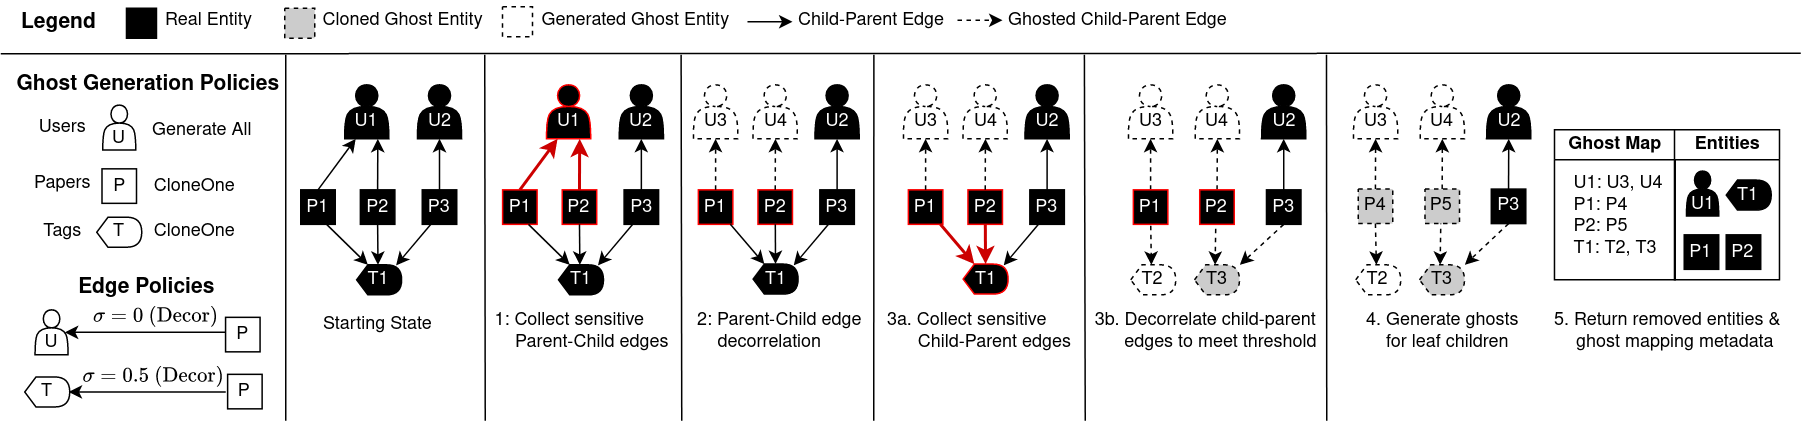
\includegraphics[width=\textwidth]{img/algo}

    \caption{Stages of \proto's execution when unsubscribing user U1. Entities and edges detected as
    sensitive are outlined in red. Only the part of the entity graph relevant to unsubscription is shown.
    For simplicity, the specified ghosting policies apply for all attributes
    of the entity: a black ghost entity indicates that it is a full clone of the original.
    New edges indicates that the edge (foreign-key) value of the child has been changed to
    point to the specified parent.\\
    In this example, \proto decorrelates paper-tag edges only enough that the proportion of sensitive papers
    is at most the sensitivity threshold of 0.5, retaining one correlation between a sensitive
    paper P2 and the parent tag T1, and decorrelating the other sensitive paper P1 from the tag.}
    \label{fig:algo}
\end{figure*}


Given an application's schema and unsubscription policy, and an entity to be decorrelated as input,
\proto executes unsubscription as follows. Figure~\ref{fig:algo} illustrates each step.
\begin{enumerate}
    \item \textbf{Parent-Child Traversal:} \proto traverses the entity graph starting from the input entity,
        going down parent to child edges (and halting if it detects a cycle). 
        \proto collects traversed edges as it traverses the graph. 
    
    \item \textbf{Parent-Child Edge Policy Application:} 
        Post-traversal, \proto acts on each collected edge instance according to the specified
        decorrelation relationship policy for that edge's type.

        \proto takes all edges of every unique parent entity, and applies policies as appropriate.
        Note that any sensitivity threshold less than $1$ requires that \emph{all} edges be decorrelated or
        deleted, depending on the developer's specified choice: all the children of this parent are
        sensitive due to the nature of \proto's parent-child traversal.

        Any edges that should be deleted removes the child entity and any descendants.
        \proto generates new ghost parents using the real parent as template for any edges that should
        be decorrelated, and rewrites the child's edge attribute to be the ghost parent's
        identifier. If any edges are retained, \proto generates a ghost parent entity to replace the
        parent.
      
    \item \textbf{Child-Parent Edge Policy Application:} 
        Next, \proto takes the children of all traversed edge instances, and considers the set of
        edges from these children to other parents \emph{not} traversed by \proto during the first
        traversal phase. In other words, these children have multiple parents, at least one of which
        is transitively connected to the input entity.

        Intuitively, children of edges traversed by \proto share a connection with the initial
        entity being decorrelated. Edges \emph{from} these children to other parent entities may
        thus leak sensitive identifying information. 

        \proto acts on these child-parent edges according to the specified edge policy for each edge's
        type. For each unique parent, \proto limits the proportion of edges of each type that connect
        to sensitive entities (the children of traversed edge instances) to below the policy's
        sensitivity threshold by either decorrelating or deleting the children. 
        If \proto retains any edges from sensitive children to the real parent, then \proto generates a
        ghost parent entity to replace the parent.
        
        Note that unlike the previous steps, this step considers edges from parents that may have
        many non-sensitive children (\eg a particular tag may correlate with many stories by various
        authors).  \proto therefore may retain edges to sensitive children when given a sensitivity
        threshold less than 1 and greater than 0, unlike in the previous step.

        \proto optionally allows developers to specify that edges have weaker or stronger edge
        policies in the child-to-parent direction than in the  parent-to-child direction. Weaker
        policies---higher sensitivity thresholds---allow \proto to retain links if \emph{only the
        child} is sensitive, but decorrelate or remove the link if \emph{both} the child and parent
        are sensitive. For example, perhaps a user wants to ensure that they are decorrelated from
        their reviews, but correlations between the review and the the paper authors can still be
        retained.

        Stronger policies may specify that the parent connected to sensitive children should
        decorrelate \emph{all} correlations to the paper even from non-sensitive correlations.
        Developers specify such a policy with a sensitive threshold of -1. For
        example, perhaps the set of users with review conflicts to the paper can identify the
        author, even if the author is decorrelated from the paper. We see an example of this in
        Section~\ref{sec:hotcrp_example} (Figure~\ref{fig:pcs}).

    \item \textbf{Anonymizing Leaf Children:}
        If any sensitive children that are leaves (have no children) remain, \proto generates a ghost child entity to replace this leaf.
        
        In Figure~\ref{fig:algo}, step 4, P1 and P2 are both leaves. \proto generates ghosts for both
        these papers: since these papers have \texttt{CloneOne} ghosting policies, ghost papers gP1
        and gP2 are identical to P1 and P2, and retain the edge attributes linking them to their
        respective parent tags and users.

    \item \textbf{Returning User Data:} \proto collects all removed entities that have either been
        replaced by ghost entities, or deleted entirely from the graph. \proto also records all
        generated ghost entity identifiers, and which ghost entities replaced which real entity.
        \proto returns both the removed entity data and this ghost entity metadata to the user.
\end{enumerate}

Note that \proto must decide \emph{which} ghost clones the template entity's attributes when the
developer selects a \texttt{CloneOne} ghosting policy for one or more attributes. \proto always
associates the cloned ghost with as many non-sensitive entities as possible. For example, as shown
in Figure~\ref{fig:algo} step 3b, if \proto decorrelates sensitive papers from a parent tag with a
\texttt{CloneOne} policy, \proto chooses the ghost tag that remains associated with non-sensitive
papers to be the clone. This decision ensures that any subscribed users and unsensitive application
data remain as unaffected as possible by another user's unsubscription. To optimize
\texttt{CloneOne} policies, \proto can simply retain the original template entity instead of producing
a cloned ghost.
\fi
%\proto provides a menu of unsubscription policy choices that allow developers to choose how to
%\emph{ghost} individual data record content, and how to \emph{decorrelate} sensitive correlations. 
%Specifying the policy requires nothing more than the application schema: ghosting policies act on
%application datatables and on foreign key relationships between tables.
%Table column values can be ghosted---removed, anonymized, or modified---in application-specific
%ways; and correlations can be broken, removed, or desensitized by adding noise. This gives
%developers the flexibility to specify fine-grained policies that properly de-identify a user, while
%retaining data as necessary for the application.

%\proto must pinpoint exactly which data and correlations may be
%identity-sensitive, and allow developers to specify exactly what the post-unsubscription state of
%this data should be.
